\documentclass{beamer}
\usepackage{tikz}
\usetheme{madrid}
\usepackage{amsthm}
\usepackage{mathtools}
\DeclarePairedDelimiter\ev{\langle}{\rangle}%
\usetikzlibrary{calc}

% \makeatletter
% \g@addto@macro\normalsize{%
%     \setlength\abovedisplayskip{-0pt}
% }
%Information to be included in the title page:
\title{Presentation: Monotone maps, sphericity and bounded second eigenvalue by Bilu, Linial}
\subtitle{CSE 269}
\author{Ian Chi}
\institute{ucsc}
\date{fall 2025}

\begin{document}

\frame{\titlepage}

\begin{frame}
\frametitle{Key results}\begin{itemize}
    \item \fbox{\begin{minipage}{0.9\textwidth}\(\delta n\) regular graphs with bounded diameter D have sphericity \(\Omega(\frac{n}{\lambda_2+1})\) where \(\lambda_2\) is the second largest eigenvalue of the adjacency matrix\end{minipage}}
    \item quasi-random graphs have logarithmic sphericity
    \item \(\frac{n}{2}\) regular graphs w/ bounded \(\lambda_2\) are \(o(n^2)\) close to bipartite graphs
\end{itemize}
\end{frame}

\begin{frame}
    \frametitle{Sphericity}
    \begin{definition}[sphericity]
        given a graph \(G\) and adjacency matrix \(A\), its sphericity is the lowest dimension \(n\) ST \(\varpi:G-\mathbb R^n\) satisfies \begin{equation}
            A_{ij}=1\iff \lvert\varphi(i)-\varphi(j)\rvert_2\leq 1
        \end{equation}
    \end{definition}

    \begin{itemize}
        \item this map would be an isometry if we used the metric on the original graph of 
        \begin{equation}\begin{split}
            &\delta^\prime(i,j) = 0 \iff i=j\\
            &\delta^\prime(i,j) = 1 \iff \delta(i,j) = 1\\
            &\delta^\prime(i,j) = 2, \text{ else}
        \end{split}
        \end{equation}
    \end{itemize}

\end{frame}

\begin{frame}
    \frametitle{Sphericity}

    \begin{equation}
        \begin{aligned}
            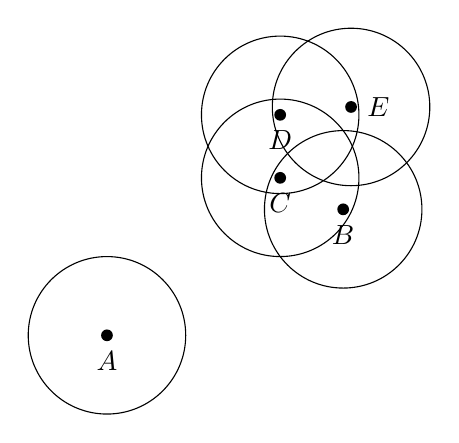
\begin{tikzpicture}
        
                % Define and draw the three points (nodes)
                \node[circle, fill, inner sep=1.5pt, label=below:$A$] (A) at (0, 0) {};
                \node[circle, fill, inner sep=1.5pt, label=below:$B$] (B) at (3, 1.6) {};
                \node[circle, fill, inner sep=1.5pt, label=below:$C$] (C) at (2.2, 2) {};
                \node[circle, fill, inner sep=1.5pt, label=below:$D$] (D) at (2.2, 2.8) {};
                \node[circle, fill, inner sep=1.5pt, label=right:$E$] (E) at (3.1, 2.9) {};
        
                % Optionally, you can connect them with lines to form a triangle
                % \draw (A) -- (B) -- (C) -- cycle;
        
                \draw (A) circle (1);
                \draw (B) circle (1);
                \draw (C) circle (1);
                \draw (D) circle (1);
                \draw (E) circle (1);
            \end{tikzpicture}
        \end{aligned}
        \implies
        \begin{aligned}
            \begin{tikzpicture}
        
                % Define and draw the three points (nodes)
                \node[circle, fill, inner sep=1.5pt, label=below:$A$] (A) at (0, 0) {};
                \node[circle, fill, inner sep=1.5pt, label=below:$B$] (B) at (3, 1.6) {};
                \node[circle, fill, inner sep=1.5pt, label=below:$C$] (C) at (2.2, 2) {};
                \node[circle, fill, inner sep=1.5pt, label=left:$D$] (D) at (2.2, 2.8) {};
                \node[circle, fill, inner sep=1.5pt, label=above:$E$] (E) at (3.1, 2.9) {};
        
                % Optionally, you can connect them with lines to form a triangle
                \draw (B) -- (C) -- (D) -- (E) -- cycle;
        
                \path (A) circle (1);
                \path (B) circle (1);
                \path (C) circle (1);
                \path (D) circle (1);
                \path (E) circle (1);
            \end{tikzpicture}
        \end{aligned}
    \end{equation}


\end{frame}

\begin{frame}
    \frametitle{spectral graph theory}
    \begin{itemize}
        \item use linear algebra/spectral theory on adjacency matricies for info
        \item \(n\) regular graphs have largest eigenvalue of \(n\)
        \item second eigenvalue gives good info on ``variance'' of edges by expander mixing lemma
        for some subset \(S,T\subset G\)
        \begin{equation}
            \left| E(S, T) - \frac{d}{n} |S||T| \right| \leq \lambda_2 \sqrt{|S||T|}
        \end{equation}
        \item \(\lambda_2\) controls for ``worst case deviation''
        \item good expander graphs lack local clusters; local clusters are easy to compress
    \end{itemize}
\end{frame}

\begin{frame}
    \frametitle{Theorem Statement}
    \begin{theorem}
        Let G be a \(d\)-regular graph with diameter \(D\) and \(\lambda_2\) be the second largest eigenvalue of \(G\)'s adjacency matrix and at least \(d-\frac{1}{2}n\). Then \(Sph(G)=\Omega\left( \frac{d-\lambda_2}{D^2(\lambda_2+O(1))} \right)= \Omega(\frac{n}{\lambda_2+1})\).
    \end{theorem}
    

\end{frame}

\begin{frame}
    \frametitle{proof}
    a couple observations:

    \begin{itemize}
        
        \item if \(X\) is real symmetric,\begin{equation}\label{rank_inequality}
            rank(X)\geq \frac{(tr(x))^2}{\sum_{i,j}^{}X_{ij}^2}
        \end{equation}
    
        \item if \(X\) is PSD, then \(\exists \) a set \(v_i\) such that \(X_{ij}=v_i\cdot v_j\). X is also called a Grammian matrix
        \item if the embedding of an enumerated graph \(w_i\in V\) is given by \begin{equation}
            \varphi:w_i\mapsto v_i
        \end{equation}
        for vectors \(v_i\) comprising of the grammian matrix \(X\), then the dimension of the embedding \(= rank(X)\)
        
    \end{itemize}
    
    \fbox{\begin{minipage}{0.9\textwidth}\textbf{Idea:}
    what we will do is construct a feasable grammian matrix where the rank is \( \frac{d-\lambda_2}{D^2(\lambda_2+O(1))} \approx \frac{n}{\lambda_2+1} \)\end{minipage}}



\end{frame}

\begin{frame}
    \frametitle{proof (cont.)}

    \begin{itemize}
        \item \(X\): nxn symmetric matrix
        \item \(J\): all ones matrix
        \item \begin{equation}
            \begin{split}
                R: (i,j)\in\mathbb R^{n\times n}\mapsto X_{ii}
            \end{split}
        \end{equation}
        \begin{equation*}
            R(X)\in \mathbb R^{n\times n}
        \end{equation*}
        rows are all the same element, \(i\)th row is just all \(X_{ii}\)
        \item \(Y\): \(2X - R(X) - R(X)^T+J\)
    \end{itemize}

\end{frame}

\begin{frame}
    \frametitle{proof (cont.)}
    \begin{itemize}
        \item why is \(Y\) like that?
    
        
    
        \begin{itemize}
            \item \(Y_{ii} = 1\)
            \item \begin{equation}\begin{split}
                    Y_{ij} &= 2\ev{x_i,x_j} - \ev{x_i,x_i} - \ev{x_j,x_j} + 1 \\
                    &= 1-\lvert x_i-x_j\rvert^2
            \end{split}
            \end{equation}
        \end{itemize} 
        \item applying rank inequality~\ref{rank_inequality}\begin{equation}
            rank(Y)\geq \frac{n^2}{n+\sum_{i\neq j}^{}\left( 1-\lvert x_i-x_j\rvert^2 \right)^2}
        \end{equation}
        \item new goal: show
        \begin{equation}\label{new_goal_1}
            \sum_{i\neq j}^{}\left( 1-\lvert x_i-x_j\rvert^2 \right)^2 = O(D^2n^2\frac{\lambda_2}{d-\lambda_2})
        \end{equation}
    \end{itemize}
\end{frame}

\begin{frame}
    \frametitle{proof (cont.)}

    \begin{itemize}
        \item we can normalize by \(D^2\). now all \(\lvert x_i-x_j\rvert\approx 1\).
        \item separate \(ij\) pairs into two groups
        \begin{itemize}
            \item \(ij\) is an edge,
            \item \(ij\) is not an edge
        \end{itemize}
        feasible embedding \(\implies\) \begin{equation}
            \begin{cases}
                \lvert v_i-v_j\rvert \leq 1 &\iff (i,j)\in E(G)\\
                \lvert v_i-v_j\rvert > 1 &\iff (i,j)\notin E(G)\\
            \end{cases}
        \end{equation}
        \item max eq~\ref{new_goal_1} \(\iff\) \begin{equation}\label{obj}
            \max \sum_{ij\notin E} \left( \lvert x_i-x_j\rvert^2-1 \right) + \sum_{ij\in E} \left( 1-\lvert x_i-x_j\rvert^2 \right) 
        \end{equation}
    \end{itemize}


\end{frame}

\begin{frame}
    \frametitle{proof (cont.)}

    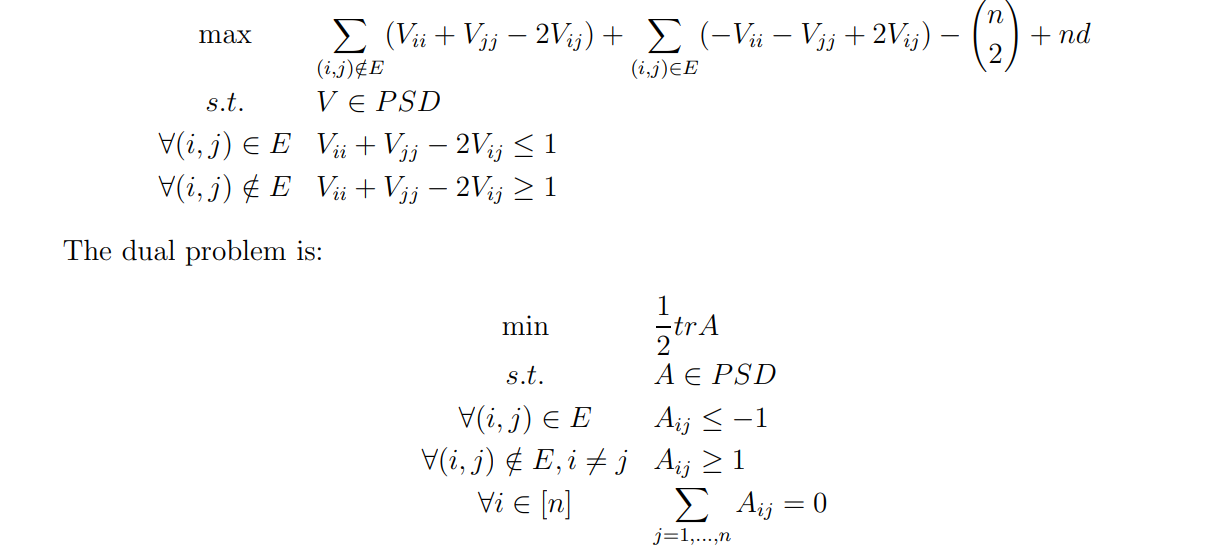
\includegraphics[width=\textwidth]{sdp_dual.png}

\end{frame}

\begin{frame}
    \frametitle{proof (cont.)}

    Create matrix that satisfies conditions for \(A\)
    \begin{itemize}
        \item the matrix \(A=(\alpha d-n)I + J -\alpha M\) where \(M\) is the adjacency matrix satisfies all of these conditions if \(\alpha>2\). 
    
        \item on edges, \(A_{ij} = 1-\alpha\), on non edges \(A_{ij} = 1\) and we want edge \(A_{ij}\) to be less than -1 by our optimization problems, thus \(\alpha\geq 2\)
        \item finally, we can check that A's eigenvalues are the same as Ms, with an eigenvector u having eigenvalue \((\alpha d-n)-\alpha\lambda_i\). to ensure this is psd, alpha is set to \(\frac{n}{d-\lambda_2}. \)
        \begin{itemize}
            \item note that \(A\vec 1 = 0\)
        \end{itemize}
        \item This \(A\) gives an upper bound on the value~\ref{obj}
    \end{itemize}

\end{frame}


\begin{frame}
    \frametitle{proof (cont.)}

    \begin{equation}
        \begin{split}
            \frac{1}{2}tr A=& \frac{1}{2}n(\alpha d-n+1)\\
            =&\frac{1}{2}\left( n^2\frac{d}{d-\lambda_2}-n^2+n \right)\\
            =& \frac{1}{2}\left( n^2\frac{\lambda_2}{d-\lambda
            _2} + n \right)
        \end{split}
    \end{equation}
    we have finished what we set out to prove in eq~\ref{new_goal_1}
    \qed

\end{frame}

\begin{frame}
    \frametitle{some results on bipartite graphs}

    \begin{equation}
        Sph(K_{m,n})\leq m+\frac{n}{2}-1
    \end{equation}
    \begin{equation}
        Sph(K_{n,n})\geq n
    \end{equation}

    \begin{center}
        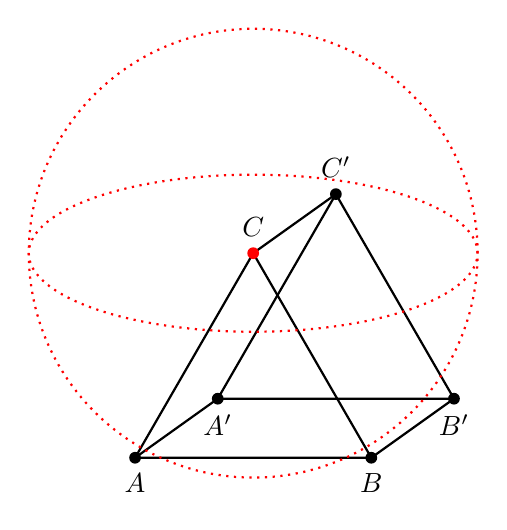
\begin{tikzpicture}[scale=3]

    % Side length of equilateral triangle
    \def\s{1}

    % Shift vector for the prism depth (same length for all three edges)
    \coordinate (shift) at (0.35,0.25);

    % Front (equilateral) triangle
    \coordinate (A) at (0,0) ;
    \coordinate (B) at (\s,0);
    \coordinate (C) at ({\s/2},{\s*0.866}); % 0.866 = sqrt(3)/2

    % Back triangle (translated by the same shift vector)
    \coordinate (A') at ($(A)+(shift)$);
    \coordinate (B') at ($(B)+(shift)$);
    \coordinate (C') at ($(C)+(shift)$);

    % Draw front face
    \draw[thick] (A) -- (B) -- (C) -- cycle;

    % Draw back face
    \draw[thick] (A') -- (B') -- (C') -- cycle;

    % Connect corresponding vertices (equal length edges)
    \draw[thick,label=below:$1+\varepsilon$] (A) -- (A');
    \draw[thick] (B) -- (B');
    \draw[thick] (C) -- (C');

    \node[circle, fill, inner sep=1.5pt, label=below:$A$] (pA) at (A) {};
    \node[circle, fill, inner sep=1.5pt, label=below:$B$] (pB) at (B) {};
    \node[circle, fill, inner sep=1.5pt, label=above:$C$,color=red] (pC) at (C) {};
    \node[circle, fill, inner sep=1.5pt, label=below:$A'$] (pA') at (A') {};
    \node[circle, fill, inner sep=1.5pt, label=below:$B'$] (pB') at (B') {};
    \node[circle, fill, inner sep=1.5pt, label=above:$C'$] (pC') at (C') {};
    
    \def\r{0.95}

    % outline of sphere
    \draw[dotted, thick, color=red] (C) circle (\r);

    % equator ellipse (3D effect)
    \draw[dotted, thick, color=red] (C) ellipse ({\r} and {0.35*\r});

    \end{tikzpicture}
    \end{center}
    


\end{frame}


\end{document}